% !TeX program = xelatex
\documentclass[a4paper]{scrarticle}

\usepackage[ngerman]{babel}
\usepackage[utf8]{inputenc}
\usepackage[T1]{fontenc}

\usepackage[left=2.25cm, right=2.25cm, top=3.00cm, bottom=3.50cm]{geometry}
\usepackage[headsepline, footsepline]{scrlayer-scrpage}
\renewcommand*{\headfont}{\normalfont}
\usepackage[backend=biber,style=apa]{biblatex} 
	\addbibresource{bibliography.bib}
	\bibliography{bibliography}
\usepackage{csquotes}

\usepackage{graphicx}
\graphicspath{ {./illustrationen/} }
\usepackage[figurename=Fig.]{caption}

\usepackage{amsmath}
\usepackage{amssymb}

\usepackage{tabto}
\usepackage{xcolor}
\usepackage{enumitem}
% \usepackage{blindtext, showframe}
\usepackage{fontspec}
\usepackage{lipsum} % for dummy text
\usepackage{siunitx}

\definecolor{AKSAcolor}{rgb}{0.64,0.44,0.32}
\newfontfamily\AKAfont{AKA}

% Redefine sectioning commands to set font
\makeatletter
\renewcommand\section{\@startsection {section}{1}{\z@}%
                                   {-3.5ex \@plus -1ex \@minus -.2ex}%
                                   {2.3ex \@plus.2ex}%
                                   {\Huge\AKAfont}}
\renewcommand\subsection{\@startsection{subsection}{2}{\z@}%
                                     {-3.25ex\@plus -1ex \@minus -.2ex}%
                                     {1.5ex \@plus .2ex}%
                                     {\Large\AKAfont}}
\renewcommand\subsubsection{\@startsection{subsubsection}{2}{\z@}%
                                     {-3.25ex\@plus -1ex \@minus -.2ex}%
                                     {1.5ex \@plus .2ex}%
                                     {\AKAfont}}
\renewcommand{\maketitle}{%
																		 \begin{titlepage}
																			 \null\vfill % Add space at the top
																			 \begin{center}
																				 {\huge\@title\par}%
																				 \vspace{0.5cm} % Adjust spacing between title and author
																				 {\large\@subtitle\par} % Add the subtitle
																				 \vspace{2.5cm} % Adjust spacing between author and subtitle
																				 
																				%  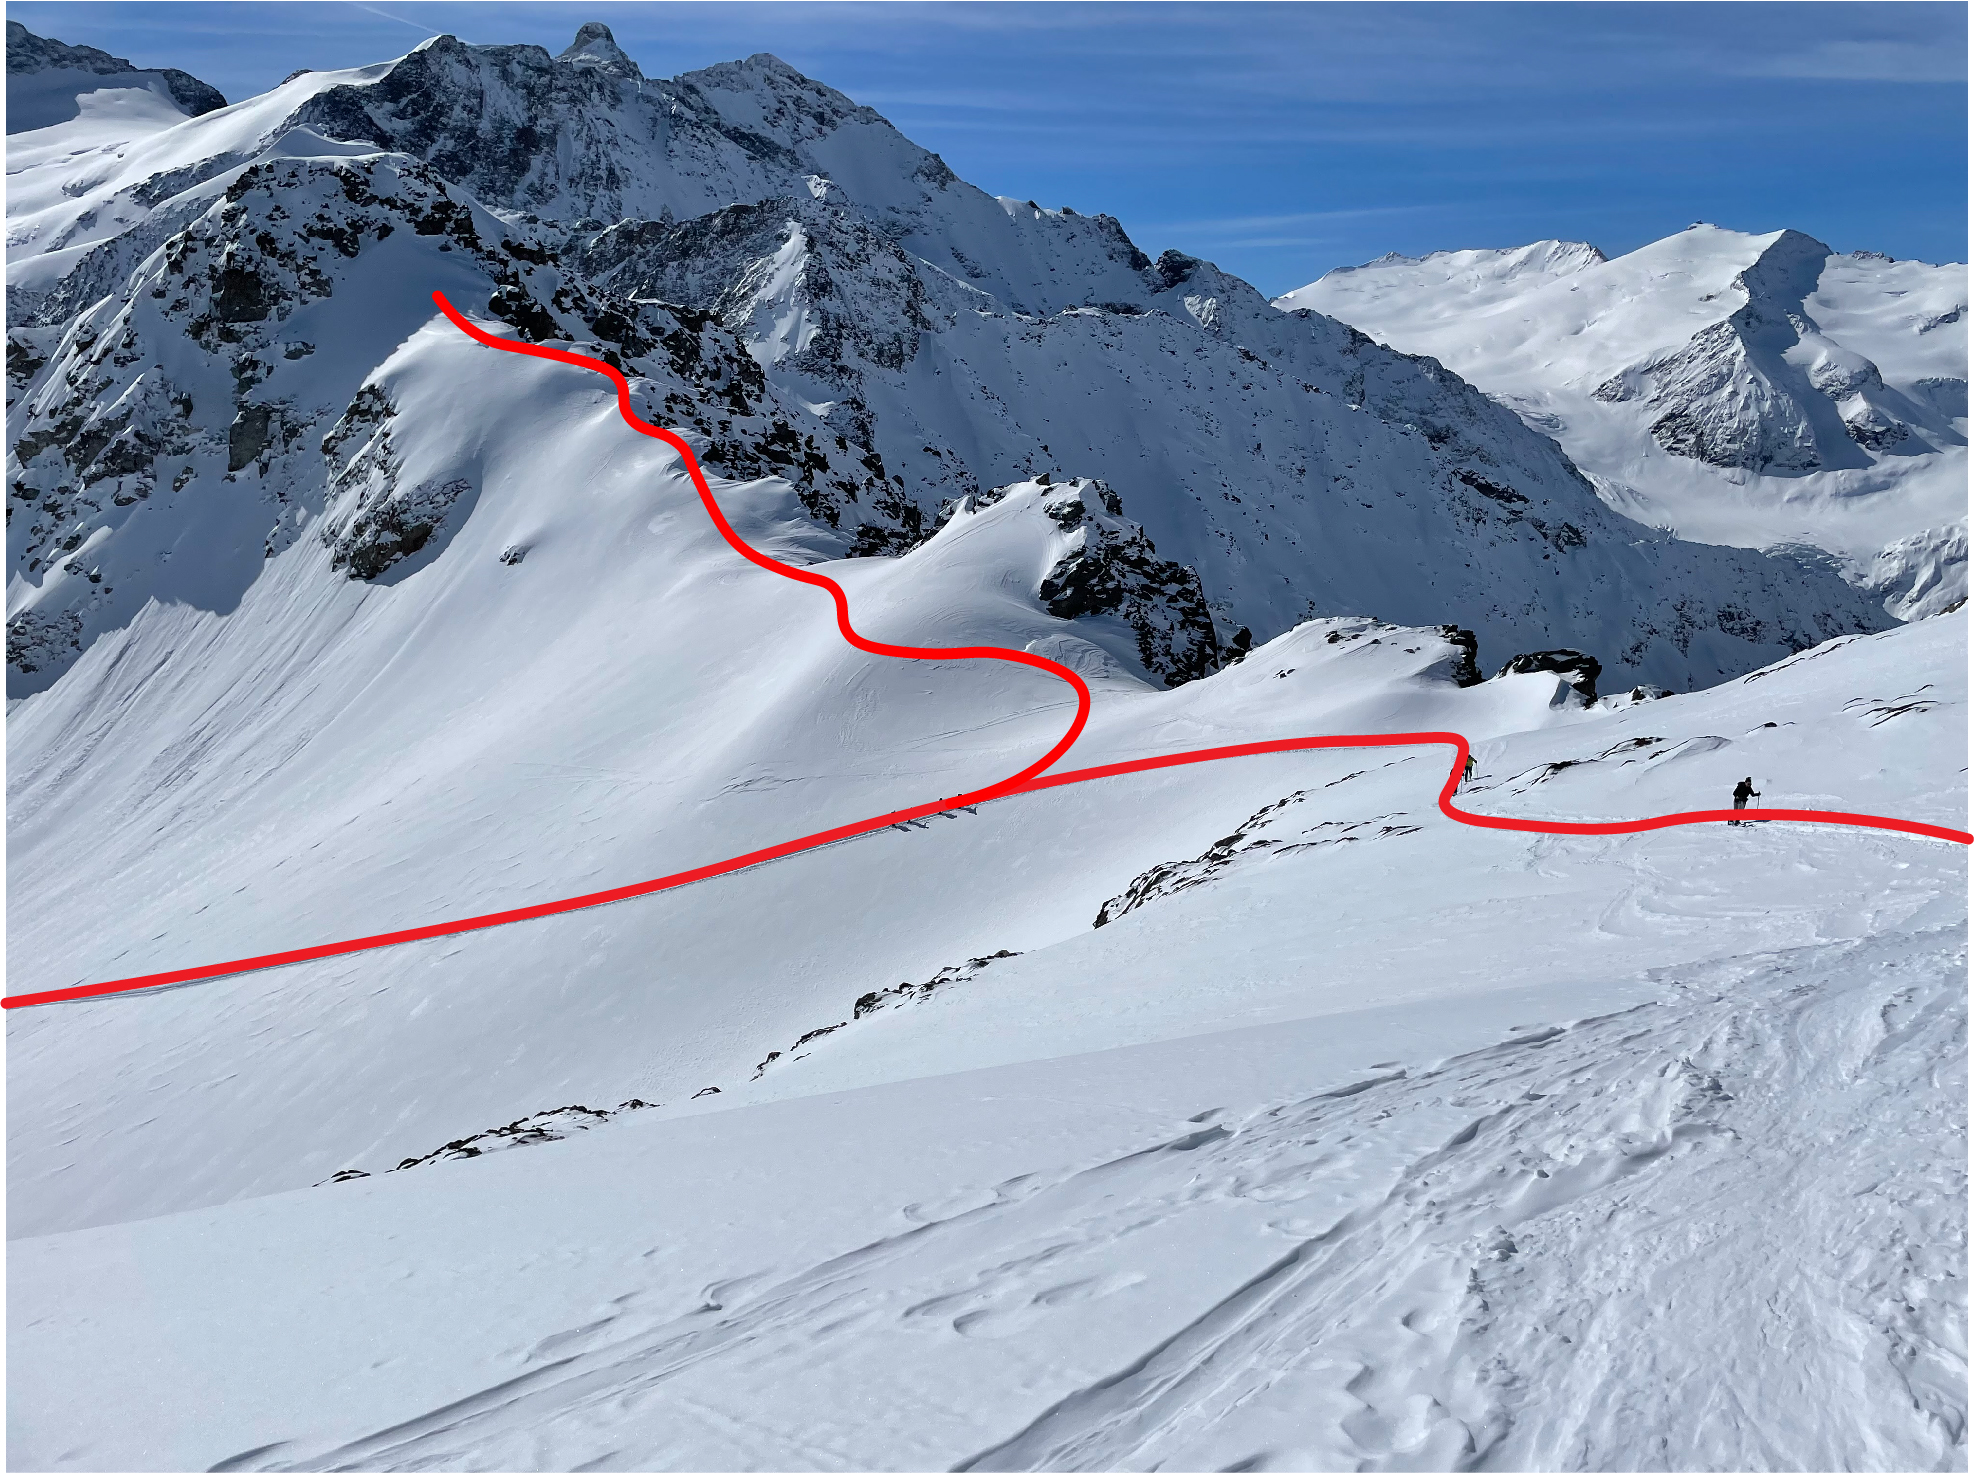
\includegraphics[width=15cm]{titelbild.png}
																				 
																				 \vspace{1.5cm} % Adjust spacing between author and subtitle
																				 {\Large\@author\par}
																				 \vspace{0.5cm} % Adjust spacing between subtitle and date
																				 {\large\@date\par} % Add the date
																			 \end{center}
																			 \vfill % Fill remaining space at the bottom
																			 \begin{center}
																				Eingereicht bei Michael Kappeler
																			 \end{center}
																			 \@thanks % If you have any thanks or notes, they will be printed here
																		 \end{titlepage}%
																	 }

\makeatother

\usepackage{hyperref}
\hypersetup{colorlinks=false, pdfborder={0 0 0}, pdftitle=}



\begin{document}

\title{\AKAfont\Huge\textcolor{AKSAcolor}{Algorithmische Skitourenplanung}}
\subtitle{Vom Bildschirm an den Berg – und zurück}
\author{Jesse Born, G21D}
\date{September 2024}

\pagenumbering{gobble} % Suppress page numbering
\ihead{Algorithmische Skitourenplanung}
\ifoot{\\Jesse Born, 2024}

\maketitle
\clearpage


\addcontentsline{toc}{section}{Inhaltsverzeichnis}
\tableofcontents
\clearpage
\addsec{Abstract}
% \addcontentsline{toc}{section}{Abstract}
In vorliegender Arbeit wird die methodische \footnote{Wie können Risikowerte berechnet werden} sowie technische Umsetzung \footnote{Wie kann ein Computer diese Berechnungen ausführen} eines Computer-Programms zur automatisierten Planung von Ski- und Bergtouren realisiert. 
\\
Auf Basis des digitalen Höhenmodels (DEM) SwissAlti\textsuperscript{3D} mit einer Auflösung von 0.5m, der Bodenbedeckungskarte SwissTLM\textsuperscript{3D} sowie historischen Unfalldaten des SLF wird eine computeroptimierte Reduktionsmethode entwickelt, welche flächendeckend individuelle Gefahrenwerte für einzelne Rasterpunkte innerhalb der Schweiz errechnen kann. Um sinnvolle Risikowerte zu errechnen, muss ausserdem die Begehungshäufigkeit zugezogen werden. (Weniger Begehungen entsprechen nicht unbedingt linear auch weniger Unfällen). Die Berechnung der Risikokarten soll dabei in Echtzeit erfolgen können, um das täglich erscheinende Lawinenbulletin sowie – als Erweiterung des Projekts – im Tagesverlauf wahrgenommene Warnzeichen in die Karte aufnehmen zu können.

Aus obigen Datengrundlagen können mittels vom Benutzer eingetragenen Start- \& Zielkoordinaten sichere, bzw. risikooptimierte Routen automatisiert geplant werden.

Ausserdem wird der Einfluss eines solchen Werkzeuges auf die Risikobereitschaft eines Tourengängers sowie dessen Nutzwert diskutiert. Die mit dem Algorithmus erstellten Routen sollen durch Bergführer, Risk-V ausgebildete Schneesportlehrpersonen sowie Freizeittourengeher blind bewertet und aus einer Auswahl von nicht-computergenerierten Routen identifiziert werden.
	

\addsec{Vorwort}
Jedes Jahr ereignen sich in den Alpen abseits der gesicherten Pisten der Skigebiete XXX tödliche verlaufende Unfälle. Fortschritte 
\clearpage
\pagenumbering{arabic}

\section{Einleitung}
\subsection{Theoretische Grundlagen}
\subsubsection{Einführung in digitale Höhenmodelle \& GIS}
Seit 20xx ist in der Schweiz das digitale Höhenmodel DHM25 verfügbar. Mit einer Auflösung von m werden aus den Höhenlinien der $1 : 25000$-Karte der Schweiz die geodätischen Höhen Computern nutzbar gemacht.
Für viele Anwendungen reicht bereits diese Auflösung aus. Fortschritte in Stereokorrelation, LIDAR und gänzlich neue Vermessungsverfahren ermöglichen heute jedoch Auflösungen unter 0.5\unit{m} mit einer Standartabweichung $\sigma \leq 0.3\unit{m}$.

\subsection{Methodik}
\lipsum[6-10]
\clearpage
\section{Hauptteil}
\subsection{Resultat}
\lipsum[6-10]
\subsection{Produktevaluation}
\lipsum[6-10]
\subsection{(Methodische Reflexion)}
\lipsum[6-10]
\clearpage
\section{Schlusswort, Fazit und Diskussion}
\lipsum[6-10]
\clearpage
\section{Literaturverzeichnis}
\lipsum[6-10]
\clearpage
\section{Abbildungsverzeichnis}
\lipsum[6-10]
\clearpage


\end{document}